% ============================================================
% Chapter 6: Results and Discussion — 本文（Phase 2, 2026-08-30）
% 骨子版（Phase 1, P1-P9）は git 履歴を参照。
% 2026-10-21 全面改訂（日本語版 8/31 報告の 2 回目の改訂 4781cdd の §4〜§9 と同じ事実・同じ数値にそろえた。
%   数値は再実験 c7c4feb の experiments/kato1020/*.json。旧値と新値は docs/加藤先生指示_2026-10-20_旧値新値対応表.md）:
%   条件: 91 件を除いた設定 A 1,732 件、第 1 段の重み (0.3, 0.7)・N_1 = 2,000、不正解は検証用で選択（19/20 で hard negative）、
%         baseline の重みは分割ごとに検証用で選択、主指標 Recall@20、R-Precision（旧 Recall@K）、検定なし（何通りの分割で
%         上回ったか）、別の出典の同じ式を正解とみなした値を併記。
%   弧: 全体比較 → 特性別 → 向上の内訳（アブレーションと PFI）→ 逐次選択 → 話題の特徴量の負の結果 → 誤り分析 → 限界。
%   削除: 旧 §6.5 自由度ゼロ停止（2026-10-14 の方針 4）、旧 §6.8 第 1 段の重みの再設計（重みは検証用で比べ (0.3, 0.7) に固定、
%         N_1 = 2,000 で被覆率 1.000 なので「介入」の前提がない）、LLM 直接生成の結果（本人の決定 2026-10-21）、
%         「飽和を予測→介入で回復」の因果の主張（新しい結果では示されない）、出典数別の分析（新しい結果にない）。
% 2026-10-21(2)（報告 f1076cd にそろえた）: 説明文 113 件の書き直しと単一出典 1 件の除外を入れた再計算が終わるまで、結果の数値は
%   1,732 件での値のまま。その旨の注記を章の冒頭に置いた（報告 §1 と同じ趣旨）。設定 A の件数は 1,731 に直した。
%   限界から「説明文が入出力変数と合っていない」を消し、定義の違う記号のあるケースを 1,299 件に数え直した。
% 2026-10-27 改訂: 再計算（8b77e73、experiments/kato1021/。説明文 113 件を書き直し core_019_v1 を外した 1,731 件）の値に差し替え、
%   冒頭の注記を消した。旧値と新値は docs/加藤先生指示_2026-10-21_説明文書き直しと92件除外_旧値新値対応表.md（設定 B は変わらない）。
%   主張の直し: §6.3 (i) は 3/10、(iii) の Recall@20 は 9/10、x10 の MAP は 9/10、§6.4 の設定 A の (3)−(2) は 7/10、
%   §6.5 の差は x7 −0.008 と合併の値、限界の重複は「除く必要がある」と言い切らず事実だけ（加藤先生の 3 回目のコメント K12）。
% ============================================================
\section{Overall Comparison}
\label{sec:overall}

Table~\ref{tab:overall} and Fig.~\ref{fig:comparison} compare the proposed method with the
classical baseline. With $N_1 = 2{,}000$, the first stage admitted every ground-truth equation of
every test case in all 10 splits (candidate coverage 1.000). The proposed method beat the baseline
on every metric, in both settings, and in all 10 splits. Static reranking raised Recall@20 from
0.906 to 0.981 ($+0.075$) and MAP from 0.693 to 0.862 ($+0.169$) in Setting~A, and Recall@20 from
0.825 to 0.966 ($+0.141$) and MAP from 0.626 to 0.832 ($+0.205$) in Setting~B. Learned greedy
selection raised MAP further, to 0.877 and 0.849 (Section~\ref{sec:greedyresults}). The variants of
the baseline with BM25 and E5 ranked no better than the TF-IDF baseline --- Recall@20 of 0.905 and
0.892 in Setting~A and 0.819 and 0.806 in Setting~B --- and the proposed method beat them, too, on
every metric in all 10 splits (\ref{app:weights}).
% source: experiments/kato1021/main.json table / compare（proposed_static vs baseline_tfidf: A Recall@20 +0.0749・MAP +0.1695、
%         B +0.1412・+0.2053、いずれも wins 10・losses 0。BM25・E5 との比較もすべての指標で wins 10）; sweep.json N1 2000 coverage 1.0

\begin{table}[h]\centering
\caption{Overall comparison (mean $\pm$ SD over 10 stratified splits). The baseline ranks the whole
database by the weighted sum of the TF-IDF text similarity and the variable overlap, with the
weights chosen on the validation cases of each split. The proposed method uses the first-stage
weights $(0.3, 0.7)$ and $N_1 = 2{,}000$ candidates. Values in parentheses count the identical
equations of other sources as correct.}
\label{tab:overall}
\footnotesize
\setlength{\tabcolsep}{3pt}
\begin{tabular}{llccc}
\toprule
Setting & Method & Recall@20 & MAP & R-Precision \\
\midrule
% source: experiments/kato1021/main.json table.A / table_equiv.A（baseline_tfidf, proposed_static, proposed_train）
A & Baseline (classical IR) & $0.906 \pm 0.020$ (0.908) & $0.693 \pm 0.061$ (0.707) & $0.607 \pm 0.059$ (0.620) \\
(1,731 cases) & Proposed, static reranking & $0.981 \pm 0.010$ (0.983) & $0.862 \pm 0.053$ (0.880) & $0.782 \pm 0.070$ (0.804) \\
 & Proposed, learned greedy & $\mathbf{0.983 \pm 0.009}$ (0.989) & $\mathbf{0.877 \pm 0.048}$ (0.906) & $\mathbf{0.811 \pm 0.070}$ (0.848) \\
\midrule
% source: experiments/kato1021/main.json table.B / table_equiv.B（説明文が変わらないので前回と同じ値）
B & Baseline (classical IR) & $0.825 \pm 0.024$ (0.827) & $0.626 \pm 0.035$ (0.636) & $0.555 \pm 0.036$ (0.568) \\
(1,000 cases) & Proposed, static reranking & $0.966 \pm 0.016$ (0.969) & $0.832 \pm 0.041$ (0.846) & $0.755 \pm 0.042$ (0.769) \\
 & Proposed, learned greedy & $\mathbf{0.971 \pm 0.014}$ (0.981) & $\mathbf{0.849 \pm 0.035}$ (0.879) & $\mathbf{0.793 \pm 0.039}$ (0.826) \\
\bottomrule
\end{tabular}
\end{table}

\begin{figure}[h]\centering
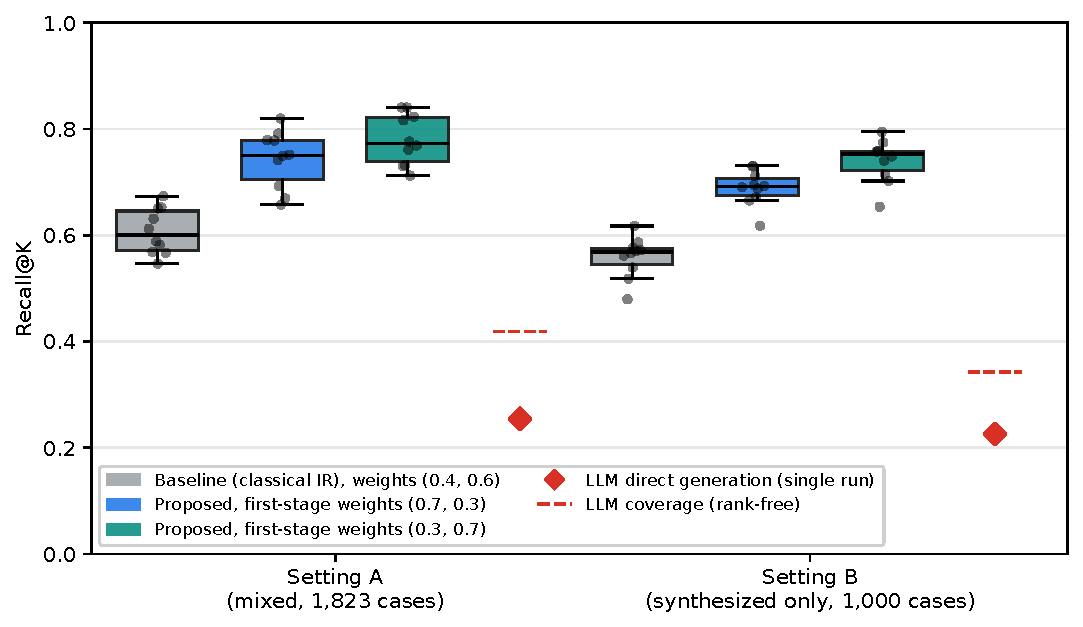
\includegraphics[width=0.95\linewidth]{figures/fig_method_comparison.pdf}
\caption{(a) Recall@20 and (b) MAP of the classical baseline and of the proposed method with static
reranking and with learned greedy selection in Settings~A and~B. Boxes show the 10 stratified
splits, and dots the individual splits.}
\label{fig:comparison}
\end{figure}

Counting the identical equations of other sources as correct (Section~\ref{sec:metrics}) raises
every method, but only a little. In Setting~A, MAP rises from 0.693 to 0.707 for the baseline,
from 0.862 to 0.880 for static reranking, and from 0.877 to 0.906 for learned greedy selection.
The gain of static reranking over the baseline in MAP hardly depends on the judgment: $+0.169$ by
identifiers and $+0.173$ with identical equations counted as correct.
% source: kato1021/main.json compare.A「proposed_static vs baseline_tfidf (equiv)」MAP +0.1731（wins 10）

The comparison with LLMs (Section~\ref{sec:compared}) has not yet run, and its results remain to
be added.

\section{Performance by Case Characteristics}
\label{sec:bycharacteristics}

Fig.~\ref{fig:characteristic} breaks the comparison down by the number of ground-truth equations
and by the number of input variables in Setting~A, pooling the test cases of the 10 splits: 4,229
records of 1,586 distinct cases (Table~\ref{tab:bucket} in \ref{app:bucket}). On the
cases with one ground-truth equation, both methods reach a Recall@20 of 1.000, and their MAP is
nearly the same: 0.931 for static reranking and 0.934 for the baseline. From two equations on, the
gap grows with the number of equations: Recall@20 differs by $+0.007$ at two equations, $+0.094$
at five, and $+0.238$ at ten. By the number of input variables, the gap in Recall@20 grows from
$+0.011$ at five or fewer to $+0.186$ at 21 or more. A variable-weighted ranking finds a single
equation as well as the proposed method does, and the lead of the proposed method grows with the
numbers of ground-truth equations and input variables.
% source: kato1021/main.json buckets.A（n_correct・n_input、延べ 4,229 件。異なるケース 1,586 件は pfi.json cancellation.gDom n_cases）

\begin{figure}[h]\centering
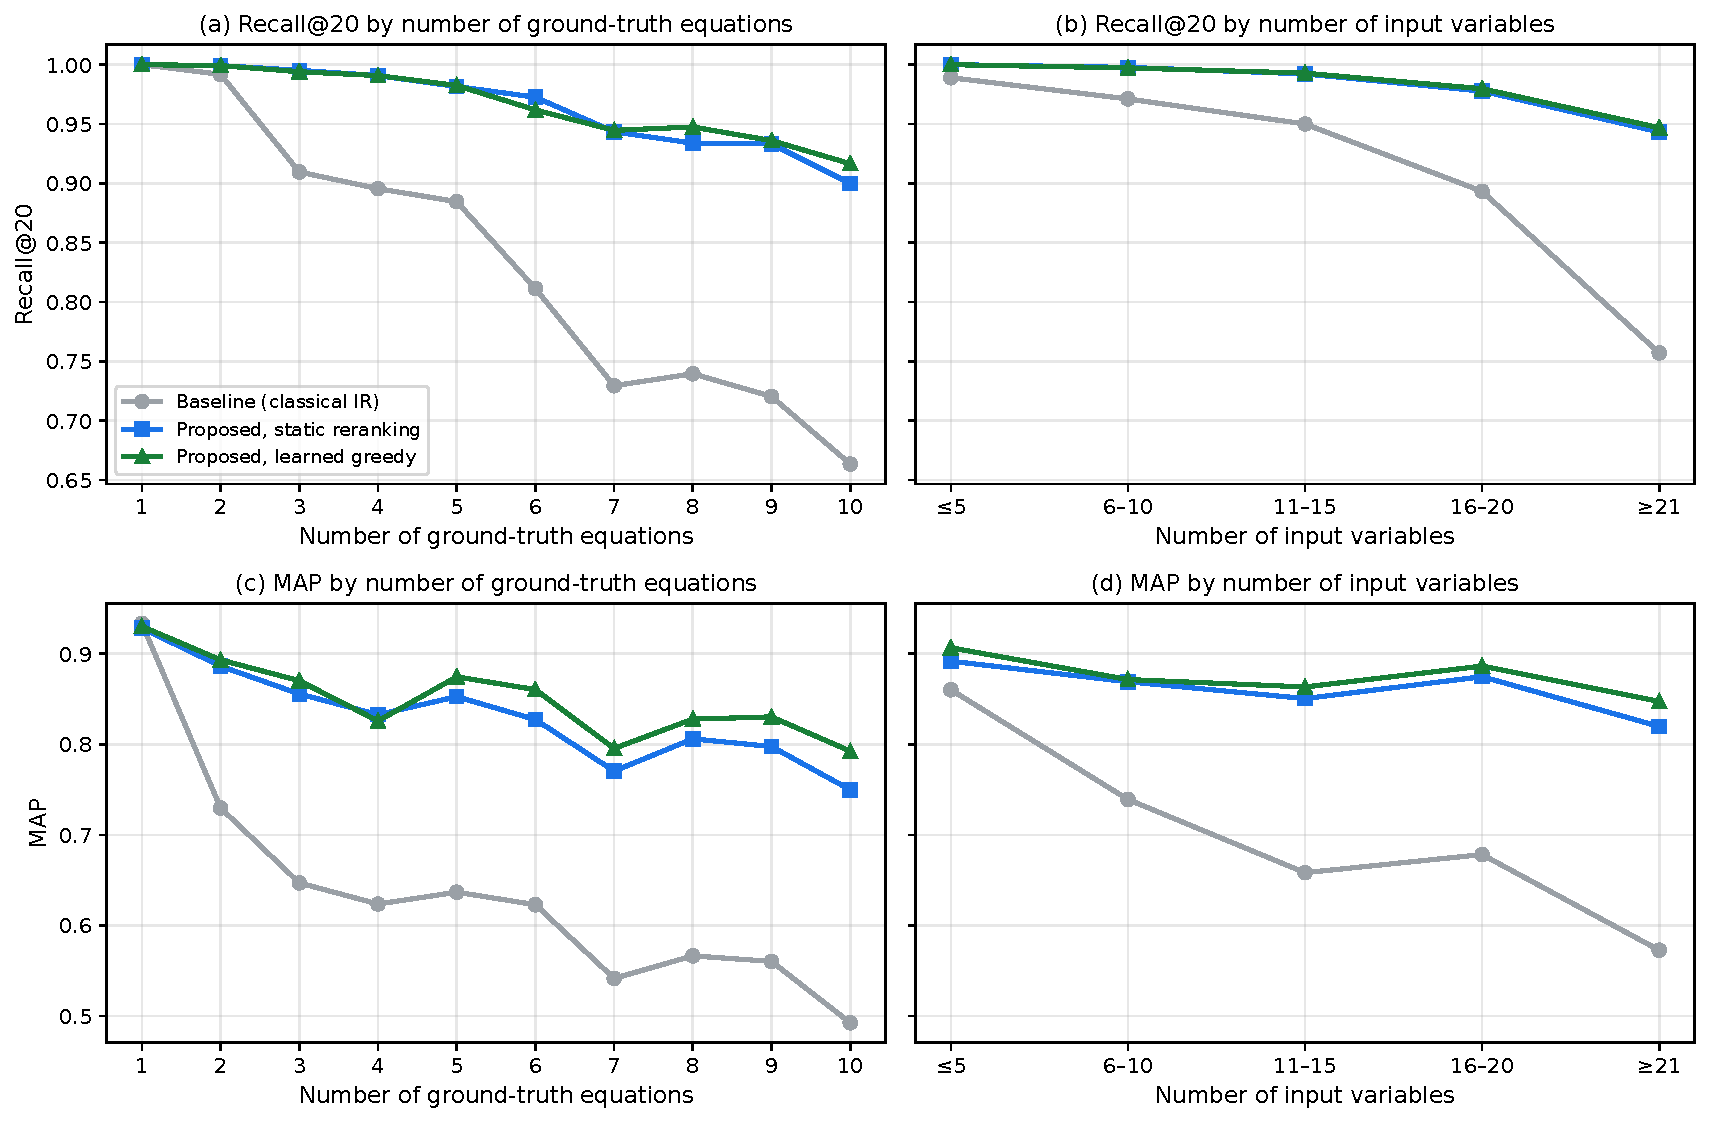
\includegraphics[width=0.95\linewidth]{figures/fig_characteristic.pdf}
\caption{Recall@20 (a, b) and MAP (c, d) in Setting~A by the number of ground-truth equations
(a, c) and by the number of input variables (b, d). Each point pools the test cases of the 10
splits (4,229 records) and carries no error bar; Fig.~\ref{fig:comparison} shows the spread across
splits of the overall values.}
\label{fig:characteristic}
\end{figure}

\section{Sources of the Improvement}
\label{sec:mechanism}

This section decomposes the gain of static reranking over the baseline with the same weights
$(0.3, 0.7)$ --- $+0.074$ in Recall@20 and $+0.169$ in MAP in Setting~A --- by growing the feature
set of the reranker, retraining it at every step, and evaluating it on the same 10 splits.
% source: experiments/kato1021/mech.json steps / summary（baseline_same_w = 重み (0.3, 0.7) の baseline: Recall@20 0.9072・
%         MAP 0.6930; total baseline_same_w → reranker-10S: +0.0738・+0.1692、wins 10）
\begin{enumerate}
  \item Learning the weights: a reranker that reads only the two Stage-1 terms, the text
    similarity $f_1$ and the I/O Jaccard $f_2$ (reranker-2), lowers Recall@20 from 0.907 to 0.904
    and MAP from 0.693 to 0.691, beating the baseline in only 3 of the 10 splits on each metric.
    Relearning how to weight the two terms does not raise the accuracy.
  \item Per-equation features: adding the other five query--equation features ($f_3$ to $f_7$)
    raises Recall@20 from 0.904 to 0.975 ($+0.071$) and MAP from 0.691 to 0.789 ($+0.098$), in all
    10 splits. Specificity $f_6$ alone carries nearly all of this step: adding it alone reaches a
    Recall@20 of 0.973 ($+0.068$) and a MAP of 0.790 ($+0.099$).
  \item Set-aware features: adding the three set-aware features to the seven raises Recall@20
    from 0.975 to 0.981 ($+0.006$, in 9 of the 10 splits) and MAP from 0.789 to 0.862 ($+0.073$, in
    all 10). Recall@20 leaves little room at 0.975, so the set-aware features mainly raise the
    ground-truth equations within the top 20.
\end{enumerate}
% source: kato1021/mech.json steps（(i) Recall@20 −0.0029 wins 3・MAP −0.0022 wins 3; (ii) +0.0711・+0.0984 wins 10;
%         (ii') +0.0684・+0.0990 wins 10; (iii) Recall@20 +0.0057 wins 9・MAP +0.0729 wins 10）
Adding the set-aware features one at a time to the seven raises MAP by $+0.073$ for
complementarity and $+0.074$ for coherence, each in all 10 splits, and by $+0.011$ for domain
agreement, in 9 of the 10. All three together add $+0.073$, no more than complementarity or
coherence alone, so the effects of these two features overlap.
% source: kato1021/mech.json single_set_additions（MAP: Comp +0.0731 wins 10・Coh +0.0736 wins 10・Dom +0.0111 wins 9）

Fig.~\ref{fig:mechanism} shows how the MAP gain of the set-aware features depends on the case. It
is $+0.007$ on the cases with one ground-truth equation, which give a candidate no other equation
to relate to, and $+0.068$ to $+0.095$ at every larger number of equations, in all 10 splits. By
the number of input variables, it is $+0.014$ at three or fewer, $+0.030$ at four to six, and
$+0.075$ to $+0.090$ at seven or more.
% source: kato1021/mech.json lift_by_n_correct / lift_by_n_input reranker-10S MAP（K=1 +0.007; K=2〜10 +0.068〜+0.095 wins 10;
%         入力 1-3 +0.014、4-6 +0.030（wins 9）、7-10 +0.087、11-15 +0.090、16+ +0.075）

\begin{figure}[h]\centering
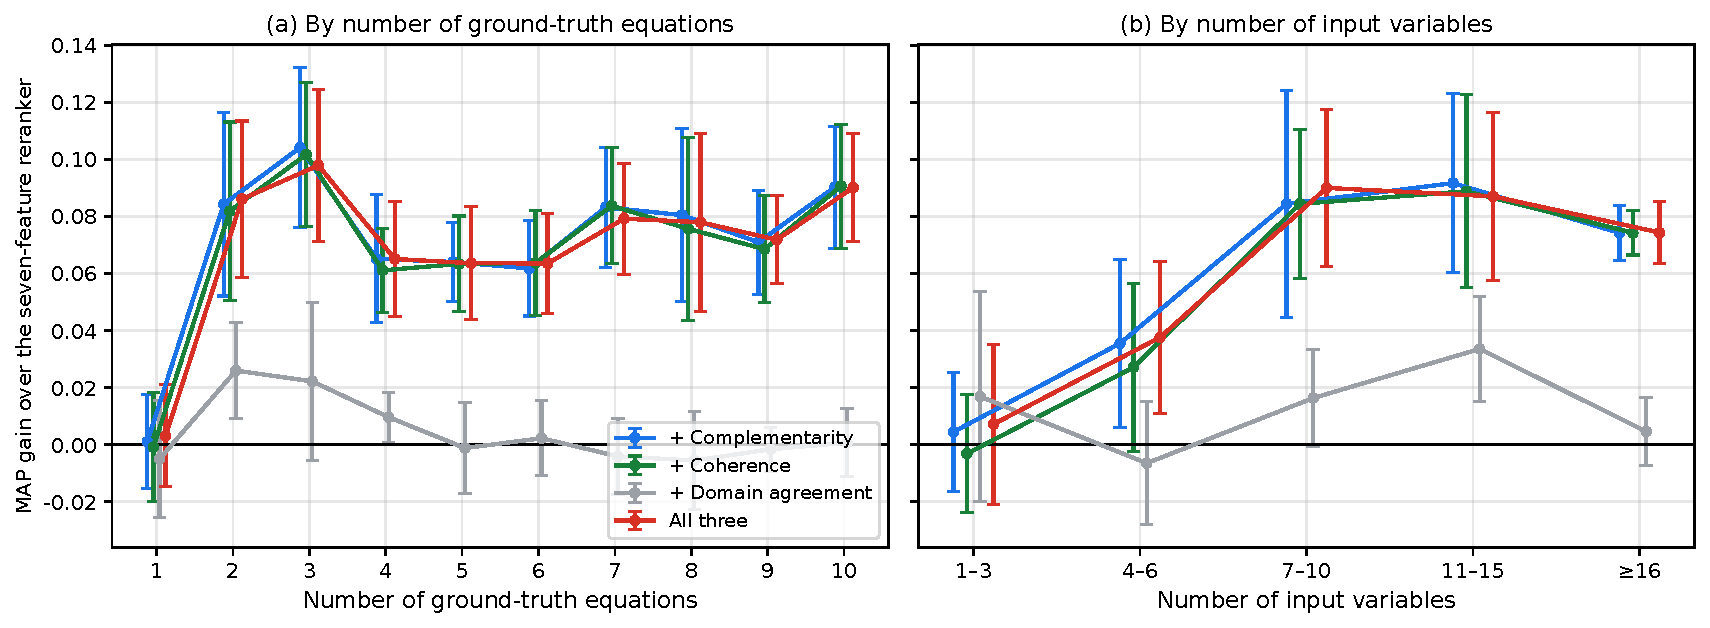
\includegraphics[width=0.95\linewidth]{figures/fig_mechanism.pdf}
\caption{MAP gain over the seven-feature reranker when the set-aware features are added one at a
time or all three together (Setting~A), (a) by the number of ground-truth equations and (b) by the
number of input variables. Points show the mean over the 10 splits of the paired difference, and
error bars its SD across the splits.}
\label{fig:mechanism}
\end{figure}

Permutation feature importance (PFI) measures, without retraining, how much the trained model
relies on each feature. We fixed the trained ten-feature model (static reranking), shuffled the
values of one feature among the candidates of each test case, and measured the drop in Recall@20
and MAP, averaging over 20 shuffles. Fig.~\ref{fig:pfi} shows Recall@20 after the shuffle.
Shuffling the six variable-overlap features ($f_2$, $f_4$--$f_6$, $g_{\mathrm{Comp}}$,
$g_{\mathrm{Coh}}$) together lowers Recall@20 from 0.981 to 0.018 and MAP from 0.862 to 0.009, in
all 10 splits. Among single features, specificity matters most: shuffling it alone lowers
Recall@20 to 0.089. Shuffling the four topic features ($f_1$, $f_3$, $f_7$, $g_{\mathrm{Dom}}$)
together leaves Recall@20 at 0.974 and MAP at 0.847; the drops, 0.007 and 0.015, are small but
appear in all 10 splits.
% source: experiments/kato1021/pfi.json（base Recall@20 0.9810・MAP 0.8622; GROUP_var → 0.0180・0.0088（低下 0.9630・0.8534、
%         正 10/10）; specificity → 0.0893（低下 0.8917）; GROUP_topic → 0.9737・0.8470（低下 0.0073・0.0152、正 10/10））
The two analyses differ in size because they answer different questions --- ablation asks what a
feature adds when the model is retrained with it, and PFI asks how much a fixed model relies on it
--- but they reach the same conclusion: the features that read variable overlap decide most of the
accuracy, and the features that read topical closeness contribute little.

\begin{figure}[h]\centering
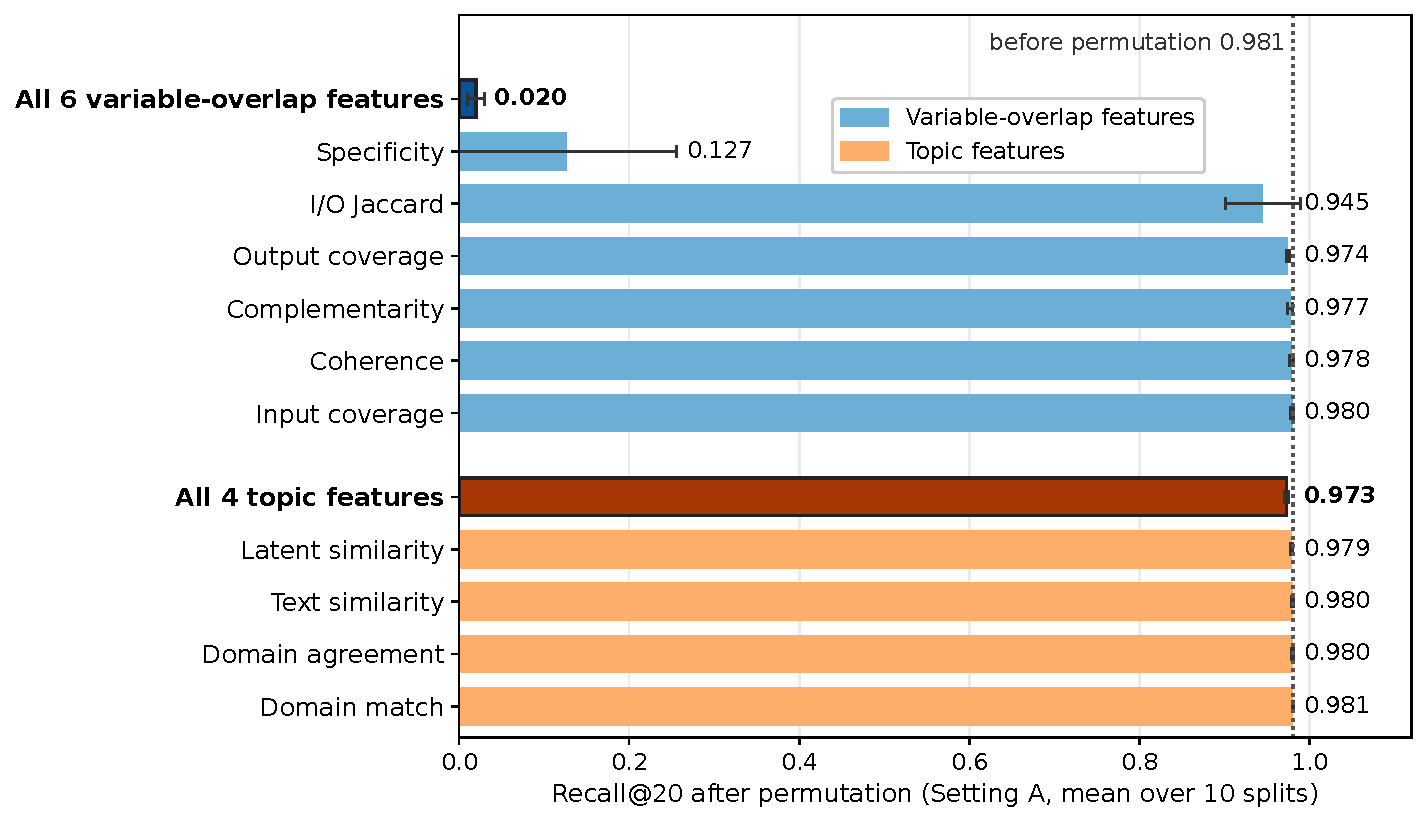
\includegraphics[width=0.78\linewidth]{figures/fig_pfi.pdf}
\caption{Recall@20 after the values of a feature are shuffled among the candidates of each case
(Setting~A, static reranking, first-stage weights $(0.3, 0.7)$, $N_1 = 2{,}000$). Bars show the
mean over the 10 splits, error bars the SD of the drop across the splits, and the dotted line the
Recall@20 before the shuffle (0.981). The first, darker bar of each group shuffles all its
features together.}
\label{fig:pfi}
\end{figure}

\section{Sequential Selection}
\label{sec:greedyresults}

Static reranking fixes the reference set to the top $m = 5$ equations of Stage~1, which drift away
from the equations that actually rise to the top when a case has many ground-truth equations. We
therefore compared (1) static reranking, (2) greedy selection at inference, and (3) learned greedy
selection (Section~\ref{sec:seq}), training and evaluating each on the same 10 splits
(Table~\ref{tab:greedy} and Fig.~\ref{fig:greedy}).

Recall@20 hardly differs among the three: about 0.98 in Setting~A and 0.97 in Setting~B. Because
the top 20 already hold nearly every ground-truth equation, the strategies differ in how they order
the equations within the top 20. MAP follows the order (1) $<$ (2) $<$ (3). Greedy selection at
inference beats static reranking by $+0.013$ in Setting~A and $+0.012$ in Setting~B, in all 10
splits of each. Learned greedy selection adds little to it: $+0.002$ in Setting~A (7 of the 10
splits) and $+0.005$ in Setting~B (9 of the 10).
% source: experiments/kato1021/greedy.json compare（all: infer − static MAP A +0.0127・B +0.0123 wins 10;
%         train − infer MAP A +0.0022 wins 7・B +0.0054 wins 9）

The differences grow on the cases with eight or more ground-truth equations, 698 test records in
Setting~A and 753 in Setting~B over the 10 splits. On these cases, learned greedy selection beats
static reranking in MAP by $+0.032$ in both settings (all 10 splits), in R-Precision by $+0.056$
and $+0.057$ (all 10 splits), and in Recall@20 by $+0.010$ and $+0.014$ (9 of 10 splits each).
Sequential selection thus pays off on the cases with many ground-truth equations, the cases that
motivated it.
% source: kato1021/greedy.json compare K>=8（train − static: A MAP +0.0321 wins 10・R-Precision +0.0561 wins 10・Recall@20 +0.0102
%         wins 9; B +0.0319・+0.0570・+0.0136, wins 10・10・9）; 延べ件数は main.json buckets（A 698、B 753）

\begin{table}[h]\centering
\caption{The three selection strategies (mean over 10 splits; $N_1 = 2{,}000$). The rows ``eight
or more'' average only the cases with eight or more ground-truth equations.}
\label{tab:greedy}
\small
\setlength{\tabcolsep}{4pt}
\begin{tabular}{llccc}
\toprule
 & & (1) Static & (2) Greedy at inference & (3) Learned greedy \\
\midrule
% source: experiments/kato1021/greedy.json summary.A / summary.B（all, K>=8）
Setting A & Recall@20 & 0.981 & 0.982 & 0.983 \\
 & MAP & 0.862 & 0.875 & 0.877 \\
 & R-Precision & 0.782 & 0.805 & 0.811 \\
 & MAP, eight or more & 0.790 & 0.816 & 0.822 \\
\midrule
Setting B & Recall@20 & 0.966 & 0.970 & 0.971 \\
 & MAP & 0.832 & 0.844 & 0.849 \\
 & R-Precision & 0.755 & 0.782 & 0.793 \\
 & MAP, eight or more & 0.785 & 0.806 & 0.816 \\
\bottomrule
\end{tabular}
\end{table}

\begin{figure}[h]\centering
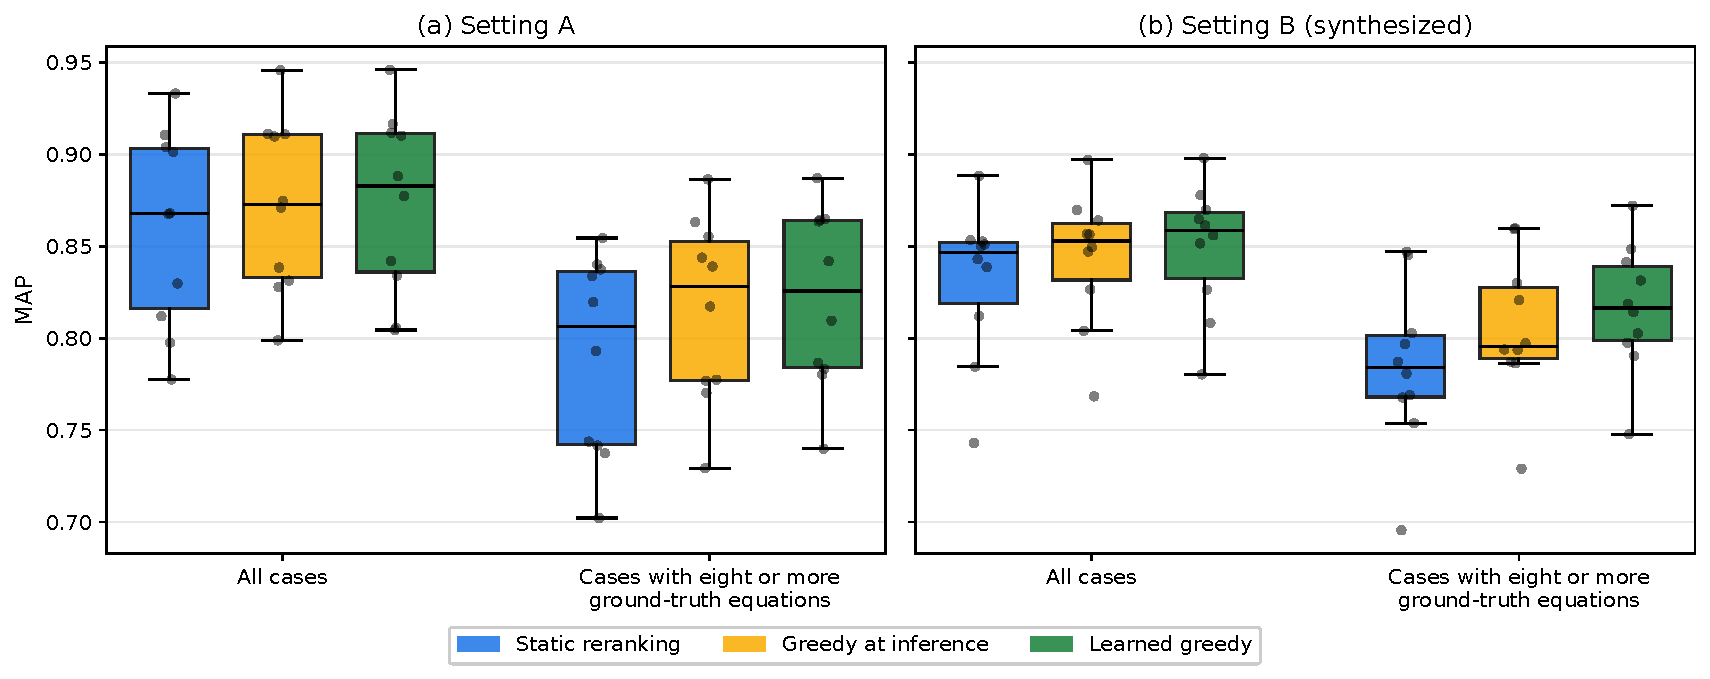
\includegraphics[width=0.95\linewidth]{figures/fig_greedy_3way.pdf}
\caption{MAP of the three selection strategies in (a) Setting~A and (b) Setting~B, on all cases
and on the cases with eight or more ground-truth equations. Boxes show the 10 splits.}
\label{fig:greedy}
\end{figure}

\section{The Null Result for Topic Similarity}
\label{sec:nullresult}

Four of the ten features read topical closeness: the text similarity $f_1$, the latent similarity
$f_3$, the domain match $f_7$, and the domain agreement $g_{\mathrm{Dom}}$
(Table~\ref{tab:features}). They rest on a reasonable expectation --- the equations of one model
should share a topic --- yet adding them did not raise the accuracy consistently in Setting~A.
Adding the domain match to reranker-2 changed Recall@20 by $-0.008$, beating reranker-2 in 5 of the
10 splits, and adding the latent similarity changed it by $-0.021$ (3 of 10). Adding the domain
agreement to reranker-7 changed Recall@20 by $-0.001$ (3 of 10) and MAP by $+0.011$ (9 of 10).
% source: kato1021/mech.json topic_additions（x7 Recall@20 −0.0076 wins 5; x3 −0.0209 wins 3; x10 Recall@20 −0.0010 wins 3・
%         MAP +0.0111 wins 9）
Coarser domain labels did not help either. We merged the labels in three ways: by unifying case,
symbols, and plural forms, which leaves 1,958 labels, and by clustering the TF-IDF vectors of the
labels with $k$-means into 100 and into 40 groups; the domain match then fires when the
description contains a label of the equation's group. Adding the domain match changed Recall@20 by
$-0.023$, $-0.028$, and $-0.030$, beating reranker-2 in 5, 4, and 3 of the 10 splits. A model with
only two or three features can lose much Recall@20 in a single split --- 0.798, against 0.931
without the domain match, in one split with the unified labels --- and such a split sways the mean
difference.
% source: kato1021/mech.json domain_merge（L1 −0.0228 wins 5; K100 −0.0275 wins 4; K40 −0.0297 wins 3）; summary の per_seed
%         （Dom@L1 の種 789 が 0.798、reranker-2 の種 789 が 0.931）; kato1014_domain_merge.py
%         （x7 を群で数える: 説明文が式の群のどれかの元のラベルを含めば 1）。2026-10-12 版の k-means の実験は、式のラベルを群の
%         名前に置き換えてから比べたため x7 がほとんど常に 0 で、合併の効果を測れていなかった（作り直した）

When the first stage keeps only 50 candidates, as an earlier configuration of this study did, two
effects contribute to the null result: the first stage leaves candidates that agree on topic, and the
selection of candidates makes the text similarity and the variable overlap correlate negatively
within them. With $N_1 = 2{,}000$ both effects nearly vanish. We measured how well one feature alone, without the
MLP, separates the ground-truth equations from the incorrect ones by the area under the
receiver-operating-characteristic curve (AUC): within each case we formed every pair of a correct
and an incorrect equation, took the fraction of pairs in which the correct equation has the higher
value (a tie counting one half), and averaged over the 1,731 cases, with the incorrect equations
drawn either from the whole database or from the 2,000 candidates (Table~\ref{tab:auc}). The latent
similarity reaches an AUC of 0.948 against the whole database and 0.909 within the candidates, so
it still separates the ground-truth equations inside the candidate set (0.594 with 50 candidates
under the first-stage weights $(0.7, 0.3)$). The correlation between the text similarity and the
variable overlap within the candidates is $-0.028$ (the 407 test cases of the split with seed 42;
$-0.404$ with 50 candidates).
% source: experiments/kato1021/topic_diag_final.json（auc_full_db / auc_within_candidates、
%         corr_text_jaccard_within_candidates_seed42_test −0.0281, n 407）; 50 件の値は kato1014_topic_diag.py を (0.7, 0.3)・
%         N_1 = 50 で回した旧 AUC 表（x3 0.594、corr −0.404。91 件を除く前の 1,823 件。
%         docs/加藤先生指示_2026-10-20_旧値新値対応表.md §8 の表 4）

The topic features still add little because the variable-overlap features alone nearly separate
the correct candidates from the incorrect ones: within the candidates, the AUC is 0.995 for the
I/O Jaccard and 0.994 for specificity, above the 0.909 of the latent similarity and the 0.849 of
the text similarity. Nor do opposing effects cancel out. Splitting the cases by whether the domain
agreement is higher on the correct or on the incorrect candidates, shuffling it lowers MAP by
0.003 in the 1,335 cases of the first kind and changes it by less than 0.001 in the 251 cases of
the second.
% source: kato1021/topic_diag_final.json auc_within_candidates（x2 0.9952、x6 0.9945、x3 0.9094、x1 0.8491）; kato1021/pfi.json
%         cancellation.gDom.MAP（n_sep_pos 1,335: 低下 +0.0026、n_sep_neg 251: 低下 −0.0001。sep = 候補の中の正解式の平均 −
%         不正解式の平均を、ケースが現れた分割で平均）

\begin{table}[h]\centering
\caption{How well one feature alone separates the ground-truth equations from the incorrect ones
(AUC; mean $\pm$ standard error over the 1,731 cases of Setting~A). The columns differ in where the
incorrect equations come from.}
\label{tab:auc}
\small
\begin{tabular}{lcc}
\toprule
Feature & Whole database (11,146 equations) & Within the 2,000 candidates \\
\midrule
% source: experiments/kato1021/topic_diag_final.json（mean ± sem、n 1,731）
I/O Jaccard $f_2$ & $0.999 \pm 0.000$ & $0.995 \pm 0.000$ \\
Specificity $f_6$ & $0.999 \pm 0.000$ & $0.994 \pm 0.000$ \\
Latent similarity $f_3$ & $0.948 \pm 0.003$ & $0.909 \pm 0.003$ \\
Text similarity $f_1$ & $0.909 \pm 0.004$ & $0.849 \pm 0.005$ \\
Domain agreement $g_{\mathrm{Dom}}$ & $0.769 \pm 0.004$ & $0.764 \pm 0.004$ \\
Domain match $f_7$ & $0.577 \pm 0.003$ & $0.573 \pm 0.003$ \\
\bottomrule
\end{tabular}
\end{table}

\section{Error Analysis}
\label{sec:erroranalysis}

We examined one split, that with seed 42: its 407 test cases hold 1,622 ground-truth equations,
and its Recall@20 of 0.974 lies below the 10-split mean of 0.981. Static reranking left 84 of the
ground-truth equations out of its top 20. The 2,000 candidates contained every ground-truth
equation, so the second stage, not the first, missed all 84. The 365 cases with every ground-truth
equation in the top 20 average 3.55 ground-truth equations and 14.1 input variables, against 7.81
and 25.8 for the 42 cases with misses. We paired each missed equation with each incorrect equation
ranked above it and counted the pairs in which the missed equation has the higher value of a
feature: 0.46 of the pairs for the latent similarity, 0.47 for the text similarity, 0.52 for
specificity, and 0.33 for the I/O Jaccard. Every fraction lies near or below one half, so the
present features cannot repair these errors.
% source: experiments/kato1021/case_outcomes_final.json top20（n_cases 407、n_gt 1,622、mean_recall 0.9739、missed 84 =
%         stage1 0 + stage2 84、solved 365 / unsolved 42、n_correct 3.545 / 7.81、n_input 14.05 / 25.83、rescue_fraction
%         svd 0.456・text 0.470・specificity 0.523・io_jaccard 0.328）

Two types of error recur among the misses of the second stage. The first is an identical equation
from another source. Standard equations appear in many documents, so the model may present an
identical copy from another source: in one batch-fermentation case, the same growth equation
$\mathrm{d}X/\mathrm{d}t = \mu X$ from another document ranked above the ground-truth one. The
evaluation identifies equations by their identifiers and counts such a copy as incorrect, although
it serves the engineer just as well. Counting the copies as correct raises the MAP of Setting~A from
0.862 to 0.880 for static reranking and from 0.877 to 0.906 for learned greedy selection
(Section~\ref{sec:overall}). The second type is the direction of an equation. The features read
only sets of variables, so two equations that determine different variables from the same
variables --- the equations for $\mathrm{d}C_A'/\mathrm{d}t$ and $\mathrm{d}T'/\mathrm{d}t$ of a
linearized reactor, for example --- take the same value on every feature. This error misleads the
engineer as well, and its repair calls for a feature that encodes which variable an equation
determines.
% source: docs/考察_特徴量の期待と結果_2026-08-09.md §5.5（dae_X1_040, dae_X1_089）; 日本語版報告 §8.2

\section{Limitations}
\label{sec:limitations}

Nine limitations qualify these results. First, language models produced parts of the data. One
wrote the descriptions of the synthesized cases, whose style may differ from requests written by
engineers, although a program fixed the equations, inputs, and outputs of those cases
(Section~\ref{sec:synth}). Another picked the ground truths of the single-source cases, which are
the sets it judged minimal, and we have not verified their minimality (Section~\ref{sec:cases}). Second, the method matches
variables by symbol alone and ignores their definitions. In 1,299 of the evaluation ground truths, a
symbol that appears in two or more
ground-truth equations carries definitions that differ between them. Most differences are
paraphrases, but a language model (Claude Opus~5.5) that compared the definitions judged that in
596 cases an input or output symbol denotes different quantities in different equations; no person
has checked these judgments.
% source: training_cases.json と unified_equations.json から実測（2026-10-21: 2 本以上の正解式に現れる記号の定義が完全一致で
%         違うケース 1,300 / 1,732。core_019_v1 を除くと 1,299 / 1,731）; experiments/var_descriptions.json（claude-opus-5-5、
%         meaning_conflict のあるケース 596。core_019_v1 を除いても 596）
Third, the evaluation is internal to the database: retrieval cannot find an equation that the
database lacks. Fourth, the evaluation judges equations by their identifiers, so an identical
equation from another source counts as an error, although we also reported the results with such
equations counted as correct (Section~\ref{sec:overall}). The database holds the same document as
several sources (36 documents) and identical equations from different documents, and identical
equations can take up several of the top 20 places. Fifth, nobody screened the documents by hand,
so some
have little to do with physical models, and a Gemini version that no record keeps extracted the
equations of the 9 earliest documents (Section~\ref{sec:db}).
% source: docs/appendix_materials/duplicate_works.csv（36 文献）
Sixth, the six variable-overlap features alone decide most of the accuracy: shuffling them costs
0.963 of Recall@20 (Section~\ref{sec:mechanism}). The construction of the data contributes to
this, because every case takes its input and output variables from the symbols of its ground-truth
equations, so the query and the answer share one notation; whether the method stays as accurate
for queries written in another notation remains untested. Seventh, learned greedy selection trains
with teacher forcing: the reference set holds ground-truth equations during training but the model's
own selections, which may include mistakes, at inference. Eighth, among the hyperparameters, we
compared no alternative values of the reference-set size $m$, the margin $\gamma$, the number of
incorrect candidates $n_{\mathrm{neg}}$, the number of epochs, or the learning rate. Ninth, the comparison with LLMs
has not yet produced results.
